\documentclass[sigconf,authordraft]{acmart}

%% \BibTeX command to typeset BibTeX logo in the docs
\AtBeginDocument{%
  \providecommand\BibTeX{{%
    \normalfont B\kern-0.5em{\scshape i\kern-0.25em b}\kern-0.8em\TeX}}}

\usepackage{algorithm}
\usepackage{algpseudocode}

\begin{document}

\title{Towards a Domain-Specific Language for Hardware In-The-Loop Testing of Mixed-Signal Embedded Systems}

%%
%% The "author" command and its associated commands are used to define
%% the authors and their affiliations.
%% Of note is the shared affiliation of the first two authors, and the
%% "authornote" and "authornotemark" commands
%% used to denote shared contribution to the research.
\author{Graham Power}
\email{powerg@mcmaster.ca}
\affiliation{%
  \institution{McMaster University}
  \city{Hamilton}
  \state{Ontario}
  \country{Canada}
}

%%
%% By default, the full list of authors will be used in the page
%% headers. Often, this list is too long, and will overlap
%% other information printed in the page headers. This command allows
%% the author to define a more concise list
%% of authors' names for this purpose.
\renewcommand{\shortauthors}{Graham Power}

%%
%% The abstract is a short summary of the work to be presented in the
%% article.
\begin{abstract}
Testing and validation of an embedded system is one of the most complex challenges of the design. While software testing has many tools to help automate this process, the electrical validation is left mainly as manual work. As such, it takes extensive human resources and time to validate successfully.
Ideally, an automated solution would be provided. However, that generally means writing code, and we find there is usually little overlap between those responsible for designing the electrical system and those who can write code. So, even more human resources and time are required to write automated tests.
In this paper, we propose a domain-specific language to allow electrical systems designers to write automated tests for their designs easily and quickly. We first focus on finding and accelerating an optimal algorithm for validating arbitrary time-series signals. Then, we implement a domain-specific language capable of auto-generating these algorithms and all supporting code. This approach greatly reduces the time and effort required to validate electrical designs for embedded systems by eliminating the need for manual validation and dedicated engineers to write automated tests.
\end{abstract}

%%
%% Keywords. The author(s) should pick words that accurately describe
%% the work being presented. Separate the keywords with commas.
\keywords{domain-specific languages, testing, validation, hardware in-the-loop}

%%
%% This command processes the author and affiliation and title
%% information and builds the first part of the formatted document.
\maketitle

\section{Introduction}

Testing and validation are critical parts of embedded systems design, especially if one wants to be confident in the functionality of the system before releasing it for public use or remote operation such as in a spacecraft \cite{DSL:CyberPhysical}, leaving a desire for many companies to automate this work without losing confidence in the validation process. Testing automation tools already exist for software applications such as the Unity test framework \cite{SW:Unity}, Pytest \cite{SW:Pytest}, and many more. But to our knowledge, no such automation solution exists for mixed-signal validation of embedded systems. This means that dedicated validation engineers are required to write these tests. However, there is a knowledge gap between those who designed the system and know how it is supposed to function and those who know how to write tests to validate its functionality. This leaves for a significant overhead in the testing and validation process of these systems \ref{fig:proc1}. Ideally, the electrical designers would have an easy way to write their own tests, eliminating this significant overhead \ref{fig:proc1}.

This paper aims to provide a domain-specific language to aid in code-generation of automated testing for arbitrary time-series signals as a step towards testing full mixed-signal embedded systems. We will be focusing on validating exponential pulses in our DSL since they both fit the bill for a mixed-signal and validation of these types of signals has real-world applications such as detector validation on spacecraft payloads like the McMaster PRESET mission \cite{PRESET}. For arbitrary time-series signals, we use dynamic time warping as our metric for signal validation as it has been shown to be a good metric for this type of application \cite{SIG:TimeSeriesCompare}. However, one challenge is to make dynamic time warping fast without losing accuracy since the original algorithm has quadratic time and space complexity \cite{SIG:AccelerateDTW}.

In this paper, we first review the existing work in accelerating dynamic time warping and in domain-specific languages for hardware testing. We then compare the relative speedups and accuracy of different DTW implementations, both against the existing UCR dataset \cite{SIG:UCRArchive2018} and a custom exponential pulse dataset. Then, we design and propose a domain-specific language for generating executable code to run these comparisons in an automated way. The design choices behind the DSL are explained, and an example program is executed. Finally, we propose future work to extend the functionality of our domain-specific language.

\begin{figure}
    \centering
    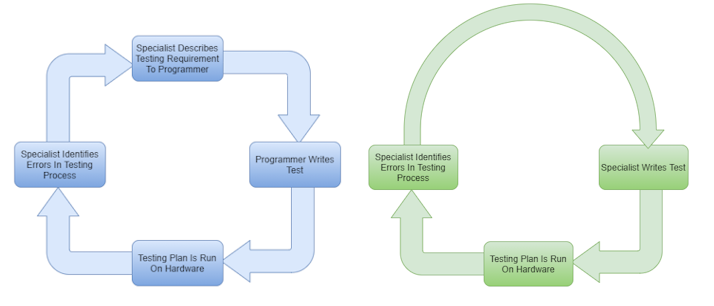
\includegraphics[width=0.8\linewidth]{img/old_process.png}
    \caption{A Comparison of the Testing and Validation Process With the Involvment of a Programmer to Write Automated Tests (Left) and With a Domain-Specific Language Useable by the System Specialist}
    \label{fig:proc1}
\end{figure}


\section{Background}

Before designing and implementing a domain-specific language for hardware-in-the-loop testing, we must choose an appropriate metric to use in our signal comparison. So, we will first look at different approaches to signal comparison and their effectiveness before exploring existing domain-specific languages.

\subsection{Signal Comparison Approaches}

Thonnessen et al. \cite{SIG:HilPLC} proposed multiple algorithms for signal validation for hardware-in-the-loop testing, such as tolerance domain and set match. While the algorithms are highly accurate, they were designed primarily for pulse-width modulated (PWM) signals or other simple digital signals. As such, they will not be reliable in a mixed signal validation environment.

Earlier, Zhang et al. \cite{SIG:WCOMP} proposed the WCOMP tool for mixed-signal validation in memory design. While the tool does provide algorithms such as pattern comparison, which uses Wiener filtering, they specifically target signals found in memory design, so it is unclear how effective these tools will be on arbitrary time series.

In a comparison work, Bagnall et al. \cite{SIG:TimeSeriesCompare} attempted to compare 19 algorithms for time series classification over 85 different problems using the University of California, Riverside time series classification archive \cite{SIG:UCRArchive2018}. They found that two algorithms consistently outperformed the others in terms of classification accuracy: Collective of Transformation Ensembles (COTE) and Dynamic Time Warping (DTW). Although COTE outperformed DTW with an average accuracy gain of 8\% over DTW, it is incredibly computationally intensive. Bagnall et al. point out that COTE is bounded by the Shapelet Transform, which has \(O(n^2m^4) \) time complexity. This is, unfortunately, unusable for the real-time signal validation required by hardware-in-the-loop testing. The second best algorithm was DTW, which has a much better, but still unideal, time complexity of \( O(nm) \). It is for this reason that DTW will be used as the basis of signal validation.

Many attempts have been made in the past to accelerate DTW. Mueen and Keogh have a seminar presentation on extracting optimal performance from DTW \cite{SIG:AccelerateDTW}. They provide many approaches to improve both the time and memory complexity DTW, some of which come at the cost of accuracy. These approaches include limiting the warping distance, deriving a lower bound on the distance reported by DTW for time series classification, early abandon of the DTW computation, and storing only partial results in the DTW cost matrix to reduce its size. These approaches and some novel ones we present will be compared in later sections of this paper.

Improvements in DTW algorithms, which trade off accuracy for speed, have also been made. Silva and Batista proposed a pruning method to replace early abandonment with an exact approach that does not trade speed for accuracy \cite{SIG:PruneDTW}. However, they only compare their speedup against DTW algorithms, such as the basic DTW and an unrealistic OracleDTW and not the early abandoned implementations they aim to replace.

The University of California, Riverside, has also spent many years generating and curating an archive of time-series data to compare the accuracy of different classification algorithms. As has been done in previous comparisons \cite{SIG:TimeSeriesCompare}. We will use this dataset to validate that our attempts to accelerate DTW do not come at the cost of accuracy loss and that DTW is a valid classification method for exponential pulses.

\subsection{Domain-Specific Languages}

Many domain-specific languages for testing embedded systems have been proposed. And while none perfectly fit our application, parts of them can be built upon to provide a complete solution for hardware-in-the-loop testing for embedded systems.

Maldonado and Garcia propose a domain-specific language to enable cloud testing of mobile applications \cite{DSL:MobileApp}. Their platform provides a clean and concise syntax, allowing for fewer lines of code to be written without the user having any cloud computing knowledge. Though this DSL is designed for testing on mass-market devices and not custom electronics, it cannot be applied to most use cases. However, their language provides a clean and simple way to describe the hardware being used in the test and has served as the inspiration for our languages' hardware description syntax.

Arrieta et al. propose automated test generation for industrial elevators \cite{DSL:Elevators}. This paper provides an incredibly detailed description of the syntax used for their language and writes very closely to a human sentence as opposed to code. This is ideal for our application, where the writer of the tests rarely has any programming background. Unfortunately, their target application is specifically industrial elevators. Although this work shows promise as something that could be generalized to support testing on arbitrary hardware, the authors have yet to do so. Their syntax, with the exception of the hardware description, was used as the basis of our language's syntax.

Barriga et al. provide a much more generalized approach to hardware testing \cite{DSL:SimulateIoT} than \cite{DSL:Elevators}. They provide a language for testing Internet of Things (IoT) devices with arbitrary sensors and actuators. Unfortunately, they only support simulation of these devices, which is not hardware-in-the-loop testing. Their work can be used as a reference for how a more application-specific language like \cite{DSL:Elevators} can be generalized to support testing of arbitrary hardware.

Shin et al. propose a domain-specific language for hardware-in-the-loop testing of cyber-physical systems \cite{DSL:CyberPhysical}. This is exactly the type of language we need, though they seem to only support simple comparisons between numbers such as equals, less than, greater than etc. and not signal matching for arbitrary time-series. For mixed-signal systems, we need the ability to compare time-series signals as well.

Finally, Anjorin et al. proposed a domain-specific language for the validation of electronic circuit designs \cite{DSL:Circuits}. However, they only do design rule checks and other pre-fabrication tests to aid in the CAD process. They do not provide a way to check the system's functionality after fabrication.

\section{Methodology}
In this section, we first attempt to accelerate DTW. We describe the acceleration approaches and the reasoning behind them, as well as our approach to validate their speedup and effectiveness. Then, we will describe the implementation of a domain-specific language to facilitate the use of DTW in hardware-in-the-loop testing for embedded systems.

\subsection{Dynamic Time Warping Implementation}

To determine the best implementation of DTW for our language, we have compared ten different implementations of DTW. Mainly from \cite{SIG:AccelerateDTW} and \cite{SIG:PruneDTW}. The full list of algorithms compared is as follows:

\begin{itemize}
    \item Original DTW (No Improvements)
    \item Swapped Loops
    \item Reduced Bitwidth
    \item Partial Cost Initialization
    \item Row/Column Threaded
    \item Row/Column Threaded Row/Column Interleaving in the Cost Matrix Memory
    \item Limited Warping
    \item Memoization
    \item Early Abandon
    \item Pruned DTW
\end{itemize}

\subsubsection{Original DTW}
This is the original DTW algorithm with no improvements. The algorithm algorithm implementation is shown in Algorithm \ref{alg:dtw}.

\begin{algorithm}
\caption{Original DTW Algorithm}\label{alg:dtw}
\begin{algorithmic}

\State $D(0:n, 0:n) \gets inf$
\State $D(0, 0) \gets 0$

\For{$i = 0; i < n; i++$}
    \For{$j = 0; j < m; j++$}
        \State $cost \gets (x(i) - y(j))^2$
        \State $lastMin \gets min(D(i-1,j), D(i,j-1),D(i-1,j-1))$
        \State $D(i,j) \gets cost + lastMin$
    \EndFor
\EndFor

\State $result \gets D(n,m)$
\end{algorithmic}
\end{algorithm}

\subsubsection{Swapped Loops}
Like in GEMM, this proposed optimization involves switching the order of the loops in Algorithm \ref{alg:dtw}. Unlike GEMM, however, swapping the loops in this case should reduce the spatial locality of the accessed cost matrix. However, since this is a relatively trivial change to make to the algorithm, it was added anyway.

\subsubsection{Reduced Bitwidth}
The exact results of the DTW algorithm are not crucial in signal matching. As long as the relative results remain the same, one should still be able to classify a time series accurately. In this approach, instead of the standard double type used in C++, we will be using the Float type, which has half the bit-width. The overall algorithm is still the same as Algorithm \ref{alg:dtw}. This should greatly improve the algorithm's speed since more of the cost matrix can now sit in a single cache line, reducing the number of cache misses from generating the matrix.

\subsubsection{Partial Cost Initialization}
When building the cost matrix in DTW, all but the first row and column of the cost matrix are overridden. Since they are never accessed before being overridden, we don't have to initialize the cost matrix fully. This new approach can be seen in Algorithm \ref{alg:pinit}

\begin{algorithm}
\caption{DTW Algorithm with Partial Cost Initialization}\label{alg:pinit}
\begin{algorithmic}

\State $D(1:n, 0) \gets inf$
\State $D(0, 1:n) \gets inf$
\State $D(0, 0) \gets 0$

\For{$i = 0; i < n; i++$}
    \For{$j = 0; j < m; j++$}
        \State $cost \gets (x(i) - y(j))^2$
        \State $lastMin \gets min(D(i-1,j), D(i,j-1),D(i-1,j-1))$
        \State $D(i,j) \gets cost + lastMin$
    \EndFor
\EndFor

\State $result \gets D(n,m)$
\end{algorithmic}
\end{algorithm}

\subsubsection{Row/Column Threaded}

DTW is fairly difficult to parallelize since the cost matrix calculations are almost entirely dependent on what came before. However, since any value of the cost matrix is dependent directly on the three values which are up and to the left of it, we should be able to calculate the cost matrix along a row and down a column in parallel without breaking this data dependency as shown in Figure \ref{fig:thread}

\begin{figure}
    \centering
    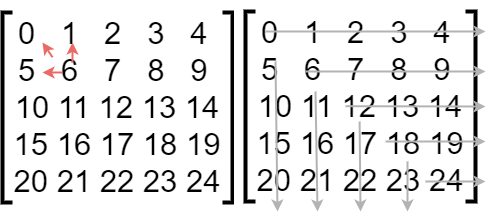
\includegraphics[width=0.8\linewidth]{img/thread_order.png}
    \caption{The Data Dependencies in the DTW Cost Matrix (Left) and the Order in Which Threads Computing Separate Rows and Columns Could be Run Without Breaking This Data Dependancy}
    \label{fig:thread}
\end{figure}

\subsubsection{Row/Column Threaded Row/Column Interleaving in the Cost Matrix Memory}
While this threading can potentially increase DTW's speed, all column threads exhibit poor cache locality, especially for larger matrix sizes. This can be solved by storing the matrix row/column interleaved. In this storage scheme, we would store the entire first row contiguously in memory, followed by the first column. This order would be repeated for all rows and columns down and to the right in the matrix. While the algorithm for calculating DTW would not change, we would need a new function for calculating the index in the memory to access given the row and column of the matrix. This function is shown in Algorithm \ref{alg:interleave}

\begin{algorithm}
\caption{DTW Algorithm with Partial Cost Initialization}\label{alg:interleave}
\begin{algorithmic}

\If{$i > j$}
\State $index \gets ((n+1)*(n))/2 + (j*n + i - 2*j - 1) - (j*(j-1))/2$
\Else
\State $index \gets (i*n + j - i) - (i*(i-1))/2$
\EndIf

\end{algorithmic}
\end{algorithm}

\subsubsection{Limit Warping}
The process of limiting the warping of DTW is described quite nicely in \cite{SIG:AccelerateDTW}. Simply, the process involves limiting the amount of distance from the main diagonal of the matrix you are allowed to go before the cost becomes infinite. To achieve this, the algorithm limits the inner loop of the basic DTW algorithm to only go +-w away from the outer loop index i, where w is the warping window.

\subsubsection{Early Abandon}
Early abandon is a method for accelerating the time to compare many time series using DTW to find the most optimal one. With early abandon, you set some lower bound for the final cost, and you are happy to accept this as a match without making further DTW comparisons. The exact value of the lower bound varies by implementation and is discussed in detail in \cite{SIG:AccelerateDTW}.

\subsubsection{Memoization and Pruned DTW}
Since both these implementations are from other papers, full details on their implementations can be found \cite{SIG:AccelerateDTW} and \cite{SIG:PruneDTW}, respectively.

\subsubsection{Domain Specific Language Implementation}

In this section, we will describe the domain-specific language we will implement, its features, syntax, and justification behind their choices. We will start by describing what the language should be like and how the syntax should look. We will then describe the method for parsing this language to produce an Abstract Syntax Tree (AST).

\subsubsection{Language Features}
Since the language will require matching time series signals to expected values, users must be able to express an arbitrary signal to use in a comparison. Allowing a mathematical representation of these signals seems the most optimal since almost any signal can be represented with a math equation. To achieve this, we must allow for basic and even complex math to be described. To achieve this, we will implement a \textcolor{purple}{MATHFUNC} keyword.

Next, we will need to support a description of the hardware being tested. We will do this with the \textcolor{purple}{HARDWARE} keyword, which allows users to describe the type of hardware connected. Every hardware definition has the following: A package name used by the compiler to determine which library functions to use. A name, preceded by the NAME keyword, gives a name to the variable. A protocol preceded by the ON keyword gives the communication protocol to use only when the package library supports multiple protocols. A pin(s), preceded by the ON keyword and protocol if it exists, gives the physical pins of the device we are using to run the test code. A conversion function, preceded by the USING keyword, provides a math function which will be used to convert all inputs/outputs to/from this hardware.

We also want the users to be able to create simple variables, both for use in mathematical equations and to provide context to the code, such as the name of the test or the author. To do this, we will provide two keywords: the \textcolor{purple}{CONSTANT} keyword for numerical constants and the \textcolor{purple}{CONTEXT} keyword for strings used to describe the code.

We also want to be able to control the output of some GPIO pins to aid in executing the test. This will be done with the \textcolor{purple}{SET} keyword.

Finally, the heart of our language is the ability to compare signals. This is done with the \textcolor{purple}{ASSERT} keyword. The user can then pass in a reference signal and a self-described signal to compare against, as well as a custom tolerance for the comparison if desired. We will support comparing both simple values with the \textcolor{purple}{EQUAL} keyword and time-series with the \textcolor{purple}{MATCHES} keyword.

A sample source code for the algorithm is shown below;

\textcolor{purple}{CONTEXT} \textcolor{blue}{NAME} = Some Testing Plan Name Here

\textcolor{purple}{CONTEXT} \textcolor{blue}{AUTHOR} = Graham Power

\textcolor{purple}{HARDWARE} \textcolor{blue}{BK2194} \textcolor{blue}{NAMED} scope \textcolor{blue}{ON} usb com4

\textcolor{purple}{HARDWARE} \textcolor{blue}{SDM3045X} \textcolor{blue}{NAMED} multimeter \textcolor{blue}{ON} usb com5

\textcolor{purple}{HARDWARE} \textcolor{blue}{GPO} \textcolor{blue}{NAMED} trig\_pulse \textcolor{blue}{ON} DIGITAL 3

\textcolor{purple}{HARDWARE} \textcolor{blue}{GPI} \textcolor{blue}{NAMED} pulse \textcolor{blue}{ON} ANALOG 5 \textcolor{blue}{USING} convert\_pulse

\textcolor{purple}{CONSTANT} Eo = 1.5

\textcolor{purple}{CONSTANT} alpha = 0.015

\textcolor{purple}{CONSTANT} beta = 0.0056


\textcolor{purple}{MATHFUNC} convert\_pulse (raw) = raw*(3.3/(212))/100/0.05*1000

\textcolor{purple}{MATHFUNC} pulse\_func (t) = Eo*(exp(0-alpha*t) - exp(0-beta*t))

\textcolor{purple}{ASSERT} multimeter \textcolor{blue}{VOLTAGE} \textcolor{blue}{EQUAL} 3.3V \textcolor{blue}{TOLERANCE} 5%

\textcolor{purple}{ASSERT} multimeter \textcolor{blue}{CURRENT} \textcolor{blue}{GREATERTHEN} 10mA \textcolor{blue}{AND} \textcolor{blue}{LESSTHEN} 600mA \textcolor{blue}{TOLERANCE} 10mA

\textcolor{purple}{SET} trig\_pulse \textcolor{blue}{HIGH}

\textcolor{purple}{ASSERT} pulse\_in \textcolor{blue}{MATCHES} pulse\_func \textcolor{blue}{TOLERANCE} 10%


\subsubsection{Language Implementation}
The language is implemented using a Recursive Descent Parser \cite{DSL:Parser} whose architecture is shown in Figure \ref{fig:parser1}. A recursive descent parser works by parsing down its structure recursively, which gives the expressions at the very bottom of the tree the highest priority when it comes to parsing. 

The bottom of our tree is built-in expressions. This is a list of keywords that map to a variable in the global space that is defined by default in the language. This allows us to easily identify and parse things like the \textcolor{purple}{CONTEXT} keyword above that we have primary expressions, which function just like any other in our language. Primary expressions consist of any variable names, numbers, or parenthesis. Above that, we have two types of math expressions: multiplicative and additive. These allow our language to support all the basic math operations like addition and subtraction. They are split into two separate nodes of the tree as an easy way to enforce an order of operations. Since the multiplicative node is below the additive in the tree, any multiplication and division will always be evaluated first when building the AST. 

Next in the tree, we have assignment expressions, which allow us to support the use of the equals sign in our language. This lets users define their own math functions or redefine context variables such as the user name and author.

Finally, at the top of the tree, we have native function calls, object expressions, and variable declarations. Native function calls are how we choose to support the assert function. Object expressions are how we define the hardware being used in the test. The \textcolor{purple}{HARDWARE} keyword indicates to the parser to create a new hardware object whose parameters are determined by the keywords following the hardware declaration. For simplicity, this language does not allow users to create custom objects. 

\begin{figure}
    \centering
    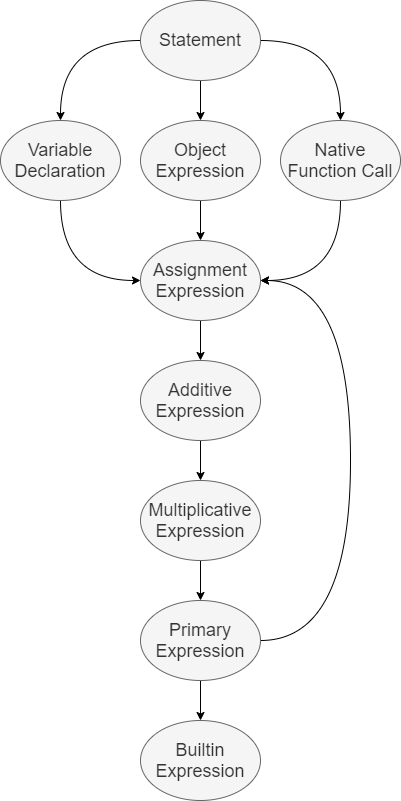
\includegraphics[width=0.8\linewidth]{img/parse_descent.png}
    \caption{The Structure of the Recursive Descent Parser Used in our Domain-Specific Language Implementation}
    \label{fig:parser1}
\end{figure}


\section{Experimental Results}

\subsection{DTW Implementation Comparison}
The accuracy of all DTW implementations was validated by running against the UCR Archive. The results can be seen in Figure \ref{fig:accuracy}. All implementations of DTW had an accuracy of around 5\%, beating out Euclidian distance, which had an accuracy of around 12\%.

\begin{figure}
    \centering
    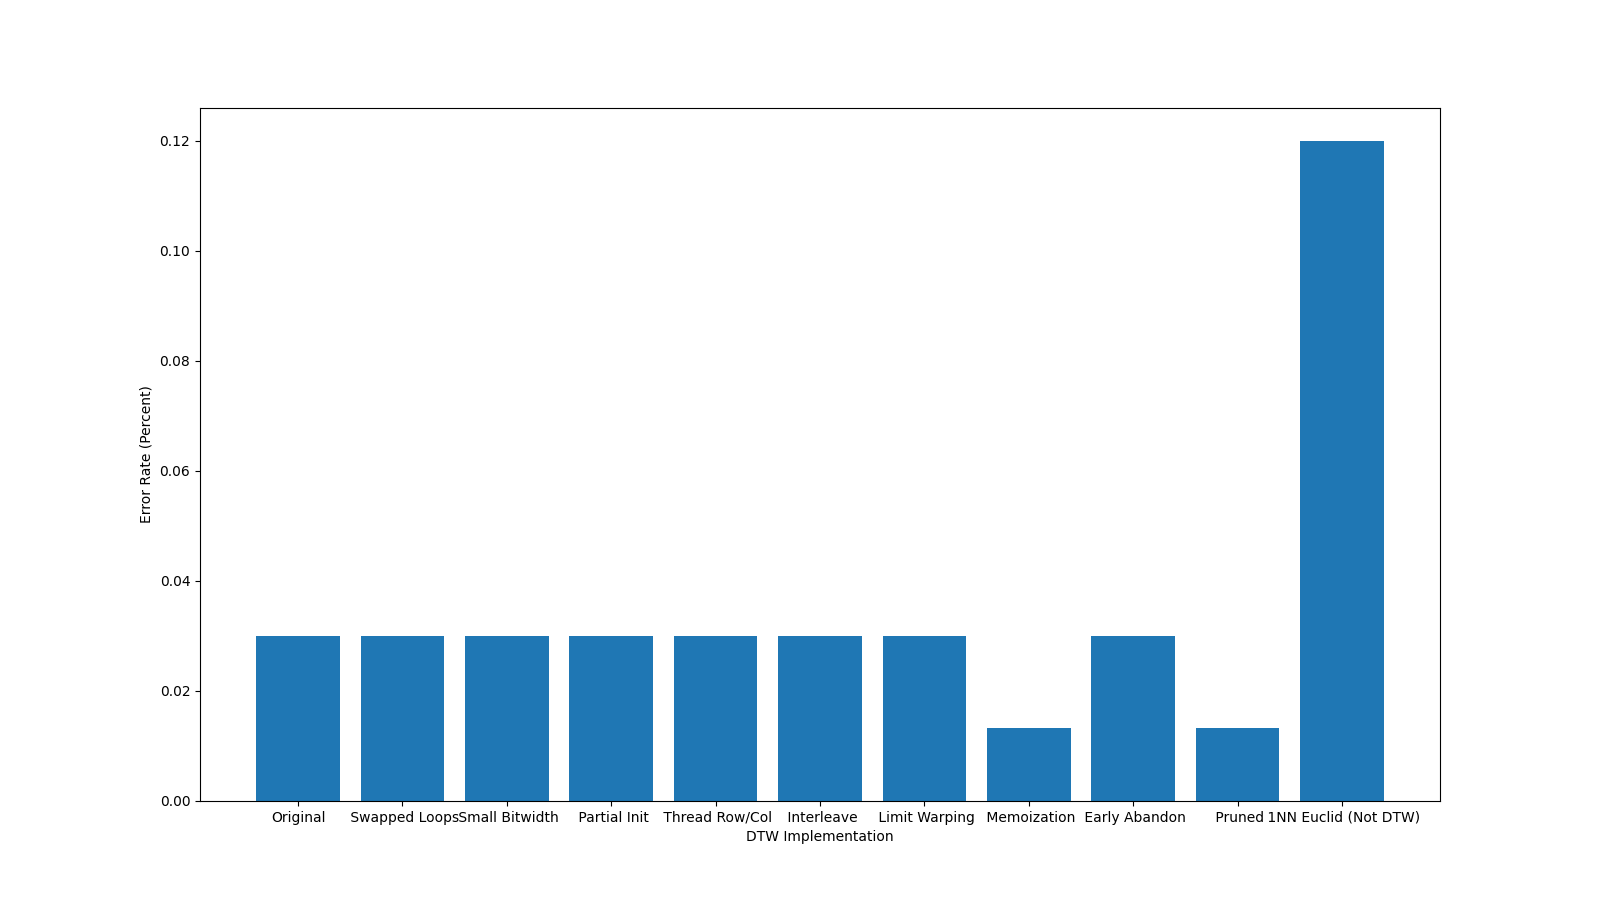
\includegraphics[width=\linewidth]{img/accuracy_results.png}
    \caption{Accuracies of Different Implementations of Dynamic Time Warping}
    \label{fig:accuracy}
\end{figure}

We also attempted to create an entry to the UCR Archive for exponential pulses, a new type of signal for their archive, and one we provided earlier in this paper as an example use case for our domain-specific language. The dataset, when tested against DTW and Euclidian distance, resulted in an error rate of around 50\% for DTW and 70\% for Euclid distance. DTW still outperformed Euclid distance, again showing it is best suited for these types of time series classifications, perhaps with the exception of COTE for non-real-time applications. 

\begin{figure}
    \centering
    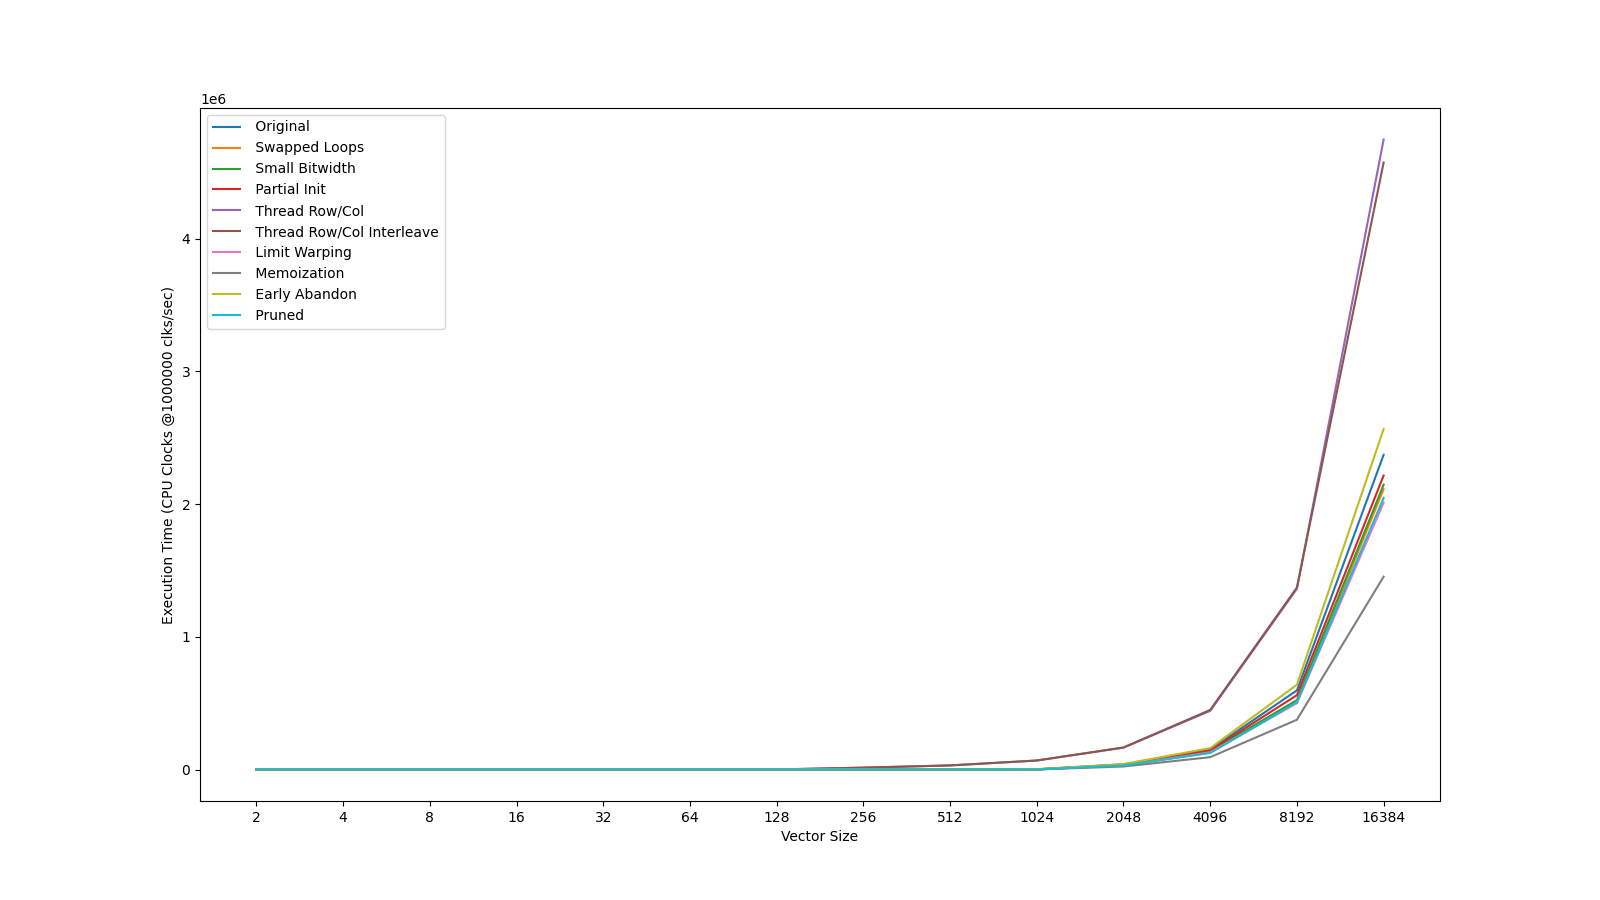
\includegraphics[width=\linewidth]{img/timing_results.png}
    \caption{Execution Time of Different Implementation of Dynamic Time Warping. Timing Results are Gathered Using the clock() Function of the Standard C++ Library, which Returns the Number of CPU Clock Ticks}
    \label{fig:timing}
\end{figure}

The last comparison of DTW algorithms was for their speedup from the base algorithm. The best implementations by far were memorization, limited warping, partial cost matrix initialization, and smaller bit-widths. Luckily, these implementations are not mutually exclusive and so could all be combined into a single implementation for use by our domain-specific language. While these implementations are faster, they still appear to scale quadratically, suggesting that running comparisons on very large vectors should be avoided for the sake of performance.

Surprisingly, our threaded application was much worse than even the original DTW implementation. This is possibly because the overhead of threading outweighs any benefit gained from having two threads running at a time. Though storing the matrix row/column interleaved did provide a performance gain over just plain multi-threading, suggesting that that approach did improve the cache locality.

\subsection{Domain-Specific Language Implementation}
The implementation of our domain-specific language consists of the following parts: A lexer to tokenize source code, a parser which generates an AST using recursive descent parsing, and a runtime which attempts to interpret and execute the AST live in Python. During the final phase of the project, I was able to implement support for all but native function calls in the parser. Unfortunately, the runtime does not support native function calls or object expressions. As a result, while I am able to generate a full AST for most of the language's proposed features, I cannot actually execute them in Python. Examples of the AST and results generated by this domain-specific language can be found in the code artifact discussed in Appendix A. The ASTs generated by the language are very verbose and would not fit neatly into a project report. 

\section{Future Work}
In the future, I would like to extend both the AST parser and runtime to support the execution of native function calls so I can show a full example of the language using DTW to compare an input signal to a mathematical model. I would also like to add support for executing the language in C or C++, so it can be run on embedded systems like an STM board and not just a Raspberry Pi.


%%
%% The acknowledgments section is defined using the "acks" environment
%% (and NOT an unnumbered section). This ensures the proper
%% identification of the section in the article metadata, and the
%% consistent spelling of the heading.
\begin{acks}
I would like to thank my instructor for this course, Dr. Kazem, for meeting with me regularly to provide valuable insights and get me on track with the course project.
\end{acks}

%%
%% The next two lines define the bibliography style to be used, and
%% the bibliography file.
\bibliographystyle{ACM-Reference-Format}
\bibliography{sample-base}

%%
%% If your work has an appendix, this is the place to put it.
\appendix

\section{Code Artifact}

The full source code for this project can be found at

https://github.com/GNPower/TestpointDSL. 

To run the code on Niagara, take the following steps:

\begin{enumerate}
  \item Clone this repository on Niagara
  \item CD to the Code/Code directory in the repository (you should see a niagara.sh file)
  \item chmod +x niagara.sh
  \item Either:
  \begin{enumerate}
        \item ./build.sh \&\& ./run.sh
        \item sbatch niagara.sh
    \end{enumerate}
\end{enumerate}

The code will produce the following results:

\begin{enumerate}
  \item The accuracy results data in Code/Code/plotGen/ accuracy\_results.txt
  \item The accuracy results graph in Code/Code/plotGen/ accuracy\_results.png
  \item The timing results data in Code/Code/plotGen/ timing\_results.txt
  \item The timing results graph in Code/Code/plotGen/ timing\_results.png
  \item The accuracy of the custom UCR Pulse Dataset in either the console or the niagara output job file
  \item The AST resulting from source code in Code/Code/ transpilerDSL/test.hil in Code/Code/transpilerDSL/test.ast
  \item The AST resulting from source code in Code/Code/ transpilerDSL/test2.hil in Code/Code/transpilerDSL/test2.ast
  \item The execution results from source code in Code/Code/ transpilerDSL/test2.hil in Code/Code/transpilerDSL/test2.res
\end{enumerate}

\section{Self Evaluation}

\subsection{Clear Problem Statement and Gap Analysis}
I believe I was able to clearly define the problem, why it exists, and how I hope to solve it. I hope to have improved since the seminar presentation since it seemed then that I had trouble getting my justification for why this is important across. Overall I would give myself 12 out of 15\%.

\subsection{Deep understanding of existing methodologies...}
I presented an in-depth analysis of the fields of both DTW acceleration and domain-specific languages for hardware-in-the-loop testing. It is this part of my project I spent the most time on researching, especially on domain-specific language implementations. I believe this is by far the strongest part of my project and would give myself 10 out of 10\%.

\subsection{A methodology that is clearly about performance optimization and automation}
I have made an attempt to propose both accelerations to the DTW algorithm, which I compare against others, and to propose a domain-specific language for automating code generation. I believe that both of these contributions fit well into the first and second sections of this course, respectively. I think my strongest part here is my proposal of a domain-specific language since, although ASTs and their uses were discussed in detail in the class, how to generate them was something I had to learn on my own from the book I referenced. Admittedly, the weaker side of my methodology was on DTW acceleration since what I was able to propose as novel only allowed for two threads running in parallel, which is far from the performance gains from something like a full GEMM optimization. For these reasons, I would give myself a 12 out of 15\%.

\subsection{An extensive experimental result that addresses your problem statement}
This is where I was the weakest. Unfortunately, my DTW acceleration attempts did not pan out as the threading overhead was much greater than the speedup expected, especially for smaller vector sizes. I also needed more time to fully implement my domain-specific language, as generating and interpreting an AST proved much harder than expected. I think the project scope was much bigger than I was reasonably able to accomplish in a single semester, especially with two courses, and I should have focused on either the domain-specific language or the DTW acceleration. For these reasons, I would give myself a 10 of 15\%.

\subsection{Presentation and technical writing quality}
I believe the presentation and technical writing quality overall to be quite good. However, there is a glaring exception. I used the sigconf template as requested, and no matter what I tried, I could not get Latex to stop generating blank pages in the middle of the paper. This has driven me crazy trying to figure it out. Besides that, I believe the technical content to be of fairly high quality. For these reasons, I would give myself a 4 out of 5\%.

\subsection{Artifact packaging}
This is the simplest one to evaluate. The code has been tested and runs well on Niagara, producing all the results I expected. So, I would give myself a 10 of 10\%.

\subsection{Overall}

Overall, I gave myself a 58 of 70\%, or an 82\% on just the project. I put a lot of work into the project over the course of the semester, and I hope it shows in the paper. However, I would not rate myself high mainly because I don't believe this is a conference-quality paper yet, and given more time, I would like to have fully implemented my domain-specific language to make my results more substantial.

\end{document}
\endinput
%%
%% End of file `sample-acmsmall-conf.tex'.
